% Auto-generated by paper/build_manuscript.py from paper/manuscript.md.
% Edit the markdown source and rerun the build script.
\documentclass[11pt]{article}

\usepackage[T1]{fontenc}
\usepackage[utf8]{inputenc}
\usepackage{lmodern}
\usepackage{microtype}
\usepackage[margin=1in]{geometry}
\usepackage{amsmath,amssymb,bm}
\usepackage{graphicx,booktabs}
\usepackage[numbers,sort&compress]{natbib}
\usepackage{hyperref}
\usepackage{xurl}
\setlength{\emergencystretch}{2em}
\setlength{\belowcaptionskip}{6pt}
\clubpenalty=10000
\widowpenalty=10000

\hypersetup{
  colorlinks=true,
  linkcolor=blue,
  urlcolor=blue
}

\providecommand{\tightlist}{%
  \setlength{\itemsep}{0pt}%
  \setlength{\parskip}{0pt}%
}

\title{Identifying a relaxing internal state in free-fall timing: finite-frequency boundaries and an application to PSR J0337+1715}
\author{Juneyoung Kim\thanks{Contact author: \href{mailto:lpaiu.cs@gmail.com}{lpaiu.cs@gmail.com}}\\{\small Independent researcher, Seoul, Republic of Korea}}
\date{28 September 2026}

\begin{document}
\maketitle

\begin{abstract}
\textbf{Proven.} We formulate finite-frequency identifiability
boundaries for a relaxing internal state in nuisance-projected free-fall
timing. At \(K\) distinct positive carrier frequencies, a nonzero single
relaxation pole admits an exact real derivative comparator of degree at
most \(N\) precisely when \(N\ge2K-1\). Positivity with a known rate gap
restricts this ambiguity. For a positive reciprocal spectrum, two
calibrated complex samples test for one observable relaxation time
through a moment-variance equality. Finite precision cannot resolve
arbitrarily close poles, and periodic observations do not determine
transients. These results specialize classical interpolation and moment
theory to timing measurements. \textbf{Counterexample candidate.} A
damped scalar-charge model supplies reciprocal forces and a controlled
one-pole reduction. \textbf{Proven.} Its leading drive in PSR J0337+1715
satisfies a phase closure violated by our earlier auxiliary analysis.
\textbf{Imported from prior work.} Auditing that analysis exposes strong
dependence on the nuisance span. A calibrated six-coefficient confidence
region gives 95.17--95.43 percent inclusion in independent simulations
within four specified covariance conditions. With archived timing
derivatives, the recorded carrier coefficients exceed its null
threshold, but an instantaneous plus single-relaxation response to the
leading physical drive fails at all six evaluated lags. Rejection is
marginal at 2 days and robust for the sign required by the scalar-charge
model. No relaxation is detected, and the excess remains unattributed.
\textbf{Conjectural.} Derivative uncertainty and incomplete physical
matching keep this conditional application from providing an empirical
strong-equivalence-principle bound.
\end{abstract}

\textbf{Keywords:} tests of gravity; strong equivalence principle;
scalar-tensor gravity; dynamical identifiability; pulsar timing

\section{Introduction}\label{introduction}

\textbf{Imported from prior work.} Compact-body structure enters
worldline effective field theory (EFT) through body-dependent
coefficients and, when needed, explicit internal degrees of freedom
\cite{goldberger2006eft,porto2016eft}. Internal modes appear as poles of
response functions
\cite{chakrabarti2013response,steinhoff2016dynamical}, and nonadiabatic
dynamical scalarization supplies a monopolar example
\cite{khalil2022scalarization}. Tests of the strong equivalence
principle (SEP) are reviewed by Will \cite{will2014confrontation}. The
pulsar triple PSR J0337+1715 has provided sensitive tests of a static
SEP parameter \cite{archibald2018universality,voisin2020sep}; a later
planet/noise analysis and public data release provide the setting for
the stored dynamic-template calculation used here
\cite{voisin2025planet,voisin2025release}.

\textbf{Proven.} A static description with finitely many operators at a
fixed order does not make a relaxing internal state unobservable, and a
pole in a body's response does not by itself make that state
identifiable from timing. A timing measurement samples the response at a
few orbital carriers, after the nuisance directions of the timing model
are projected out. Identifiability then depends on the number of
carriers, the comparator class admitted for the instantaneous response,
the nuisance span and the precision.

\textbf{Counterexample candidate.} We use a one-state relaxation as the
benchmark and a damped scalar charge as its physical realization.

\textbf{Proven.} For this benchmark we give an exact boundary for real
derivative comparators that interpolate a single pole at K carriers
(Section 3.1), a comparator restriction from positivity and a rate gap
(Section 3.2), a two-sample test and recovery of one observable
relaxation time with its finite-precision limit (Section 3.3), the
insufficiency of a finite periodic record for transients (Section 3.4),
and a phase gate on the physical drive in J0337 (Section 4). These
boundaries specialize classical results, recalled below; what is new is
their formulation for a nuisance-projected free-fall timing measurement,
the comparator classes fixed by conservative or reciprocal dissipative
physics, the drive phase gate, and their application to a stored J0337
analysis. They do not establish a new theory of gravity or a general
unobservability theorem.

\textbf{Imported from prior work.} Theorem 1 is real-coefficient
polynomial interpolation at conjugate nodes, a special case of rational
interpolation and realization \cite{mayo2007realization}, and it matches
the count by which K sinusoids are persistently exciting of order 2K in
system identification \cite{ljung1999system}. The moment-variance
inequality is the positivity of a \(2\times2\) Hankel matrix in the
truncated Stieltjes moment problem, whose singular case forces a single
atom \cite{schmudgen2017moment}. The close-pole limit is the
ill-conditioning familiar from relaxation-spectrum inversion
\cite{honerkamp1989relaxation}, and the transient obstruction is a
statement of insufficient excitation.

\textbf{Imported from prior work.} We apply them to our earlier stored
J0337 analysis, which is unpublished and recorded in the repository,
exposing the dependence of its interval on the nuisance span and
calibrating its inference (Section 5). The Supplementary Information
(Online Resource 1, abbreviated SM) contains the complete technical
account: a finite static operator catalog, the full audits and their
provenance, and a worked calculation for the inner white dwarf of the
triple. The SM keeps its own section, equation, table and figure
numbering.

Each scientific paragraph or result carries a status label.
\textbf{Proven} denotes conditional mathematics, including numerical
evaluation of explicit algebraic identities; \textbf{Imported from prior
work} denotes literature or numerical experiments recorded in the
repository, including this paper's unpublished audits;
\textbf{Counterexample candidate} denotes a proposed physical/model
realization of a state that a static description would miss;
\textbf{Conjectural} denotes an interpretation requiring additional
work. A theorem's premises are hypotheses of its conditional statement,
not independently established facts.

\section{Benchmark and comparators}\label{benchmark-and-comparators}

\textbf{Counterexample candidate.} Let a known dimensionless drive F
excite a dimensionless state and a scalar readout q:

\begin{equation}
\tau_\chi\dot\chi+\chi=\alpha F(t),\qquad
q(t)=c_YF(t)+c_\chi\chi(t),\qquad
\beta=\alpha c_\chi,\quad\tau_\chi>0,
\label{eq:model}
\end{equation}

with settled transfer function

\begin{equation}
G(i\omega)=c_Y+\frac{\beta}{1+i\omega\tau_\chi}.
\label{eq:response}
\end{equation}

The readout may correct a specified observable coupling; assigning it to
a mass or to a pairwise gravitational parameter are different modeling
choices. Relaxation presupposes an effective dissipative setting. The
general solution also contains \(\chi_he^{-(t-t_0)/\tau_\chi}\); the
periodic analysis assumes that this transient has decayed or is absent.

\textbf{Proven.} A degree-N derivative comparator is a real polynomial
\(P_N(i\omega)\), the transfer function of a local readout
\(\sum_{n\le N}a_nF^{(n)}\) with real \(a_n\). Expanding Equation
(\ref{eq:response}) in \(i\omega\tau_\chi\) gives such comparators with
error at most \(|\beta|\rho^{N+1}\) on \(|\omega\tau_\chi|\le\rho<1\),
so in the adiabatic regime a relaxation is absorbed by a derivative
comparator. The results below concern finitely many carriers at
arbitrary \(\omega\tau_\chi\).

\section{Finite-frequency
identifiability}\label{finite-frequency-identifiability}

\subsection{Exact interpolation
boundary}\label{exact-interpolation-boundary}

\textbf{Proven. Theorem 1 (real finite-frequency boundary).} Suppose
\(c_Y,\beta\) are real, \(\beta\ne0\), \(\tau_\chi>0\), and
\(\omega_1,\ldots,\omega_K\) are distinct positive frequencies at which
the drive is known and nonzero, so that the values \(G(i\omega_k)\) are
available. A polynomial \(P_N(z)\) of degree at most N with freely
chosen shared real coefficients matches \(G(i\omega_k)\) at all K
frequencies if and only if \(N\ge2K-1\).

\textbf{Proven.} Define \(R(z)=(1+\tau_\chi z)[P_N(z)-c_Y]-\beta\). Real
coefficients imply that a root at \(i\omega_k\) is accompanied by
\(-i\omega_k\). Matching thus gives 2K distinct roots, but R has degree
at most N+1. If \(N<2K-1\), R would be identically zero, contradicting
\(R(-1/\tau_\chi)=-\beta\ne0\). Conversely, set

\begin{equation}
Q_K(z)=\prod_{k=1}^K(z^2+\omega_k^2),\qquad
P_{2K-1}(z)=c_Y+
\frac{\beta[1-Q_K(z)/Q_K(-1/\tau_\chi)]}{1+\tau_\chi z}.
\label{eq:interpolant}
\end{equation}

The numerator vanishes at \(-1/\tau_\chi\), giving a real polynomial of
degree 2K-1 upon division. At every carrier it equals G. The
construction allows unrestricted coefficients; power-counting bounds,
passivity or external calibration would define a smaller comparator
class.

\textbf{Proven.} The first exact obstruction to a real degree-N
comparator is \(K=\lfloor(N+1)/2\rfloor+1\). Three positive carriers
exclude N up to four, but a fifth-degree real comparator interpolates
them. With complex coefficients and only positive-frequency samples,
interpolation permits K up to N+1. No finite polynomial equals a nonzero
single-pole response on an open frequency interval. Exact
noninterpolation does not guarantee detectability: nearly coincident
carriers or small \(\omega\tau_\chi\) can make the difference
arbitrarily small, so precision and nuisance geometry are additional
requirements.

\subsection{A comparator restriction from positivity and a rate
gap}\label{a-comparator-restriction-from-positivity-and-a-rate-gap}

\textbf{Proven.} A real local conservative quadratic action
\(\frac12\int F P(D)F\,dt\), with \(D=d/dt\) and vanishing boundary
variations, contributes the self-adjoint response \([P(D)+P(-D)]/2\), so
odd derivatives cancel. An even comparator is therefore justified for
this time-reversal-invariant conjugate response. Dissipation,
nonconjugate readout, a time-dependent background or an unknown drive
phase can invalidate this restriction.

\textbf{Counterexample candidate.} A different comparator class follows
from positive quadratic state energy, reciprocal forcing/readout and
positive Rayleigh dissipation:

\begin{equation}
\boldsymbol\Gamma\dot{\boldsymbol q}+\boldsymbol K\boldsymbol q=\boldsymbol b F,
\qquad q_{\rm out}=\boldsymbol b^T\boldsymbol q+c_0F.
\label{eq:fast-gradient}
\end{equation}

Both matrices are real symmetric positive definite. Impose a lower bound
\(\Lambda\) on every eigenvalue of
\(\boldsymbol\Gamma^{-1/2}\boldsymbol K\boldsymbol\Gamma^{-1/2}\). This
describes modes that relax faster than a specified scale; the gap is a
hypothesis requiring independent physical matching.

\textbf{Proven.} Orthogonal diagonalization gives

\begin{equation}
H(z)=c_0+\sum_j\frac{a_j}{1+z\tau_j},\qquad
a_j\ge0,\quad 0<\tau_j\le\Lambda^{-1}.
\label{eq:positive-spectrum}
\end{equation}

For \(\omega_h>\omega_l>0\), put
\(S(\omega)=-\operatorname{Im}H(i\omega)/\omega\). Then

\begin{equation}
S(\omega_l)\le R_\Lambda S(\omega_h),\qquad
R_\Lambda=\frac{1+(\omega_h/\Lambda)^2}{1+(\omega_l/\Lambda)^2}.
\label{eq:gap-witness}
\end{equation}

Indeed \((1+\omega_h^2\tau^2)/(1+\omega_l^2\tau^2)\) increases with
positive \(\tau\); summing its bound with the nonnegative weights
\(a_j\tau_j/(1+\omega_h^2\tau_j^2)\) proves the inequality. A positive
single pole with \(\tau_\chi>\Lambda^{-1}\) violates it, and the real
instantaneous coefficient cancels from S. The argument also applies to a
convergent nonnegative distribution of relaxation times with the same
support.

\textbf{Proven.} This ties the comparator to energy, reciprocity and a
rate gap rather than to an arbitrary Taylor cutoff. Negative residues, a
different drive/readout pair, oscillatory modes or removal of the gap
can evade it. Rejecting this class would not identify one internal
state: multiple slow states or a slow memory distribution can also
violate the inequality. Neither the rate gap nor reciprocal readout has
been empirically established for J0337 here.

\subsection{One observable pole from two calibrated
samples}\label{one-observable-pole-from-two-calibrated-samples}

\textbf{Proven.} Suppose
\(H(i\omega)=c_0+\int a(d\tau)/(1+i\omega\tau)\), with real \(c_0\) and
a nonnegative finite measure on \(\tau>0\). At two calibrated
frequencies \(0<l<h\), let
\(S_\omega=-\operatorname{Im}H(i\omega)/\omega\) and define

\begin{equation}
R=\frac{h^2S_h-l^2S_l}{h^2-l^2},\qquad
D=\frac{\operatorname{Re}H(il)-\operatorname{Re}H(ih)}{h^2-l^2},\qquad
Q=\frac{S_l-S_h}{h^2-l^2}.
\label{eq:positive-moments}
\end{equation}

These are the zeroth, first and second moments of
\(d\mu=\tau a(d\tau)/[(1+l^2\tau^2)(1+h^2\tau^2)]\). Therefore

\begin{equation}
RQ-D^2=R^2\operatorname{Var}_{\mu/R}(\tau)\ge0.
\label{eq:positive-single-pole}
\end{equation}

For \(R>0\), equality holds exactly for one observable relaxation time
\(\tau_0=D/R\). Its amplitude is
\(a_0=R(1+l^2\tau_0^2)(1+h^2\tau_0^2)/\tau_0\), and either real part
fixes \(c_0\). A relaxation-time atom at \(\tau=0\) would be
indistinguishable from \(c_0\). This assumes exact common drive/readout
calibration; it is not an observed equality in J0337.

\textbf{Proven.} One observable pole does not count hidden, unexcited or
degenerate internal variables. Two positive poles at
\(\tau_0\pm\epsilon\), each of weight \(a_0/2\), differ from one pole by

\begin{equation}
\frac{a_0}{2}\left[\frac{1}{1+s(\tau_0-\epsilon)}+\frac{1}{1+s(\tau_0+\epsilon)}\right]-\frac{a_0}{1+s\tau_0}
=\frac{a_0s^2\epsilon^2}{(1+s\tau_0)[(1+s\tau_0)^2-s^2\epsilon^2]}.
\label{eq:close-poles}
\end{equation}

For \(0<\epsilon<\tau_0\) both modes are stable, and the difference
vanishes quadratically. A finite-noise test cannot uniformly distinguish
exactly one pole from arbitrarily close two-pole alternatives without a
separation or weight condition. Without positivity, the stable strictly
proper addition \(\eta\prod_k(s^2+\omega_k^2)/(s+\lambda)^{2K+1}\),
\(\lambda>0\), vanishes at every carrier but changes the response
elsewhere; it need not be a positive reciprocal spectrum.

\subsection{Transients outside a finite periodic
record}\label{transients-outside-a-finite-periodic-record}

\textbf{Proven.} A homogeneous amplitude decays to fraction \(\epsilon\)
only after \(\tau_\chi\log(1/\epsilon)\); without an initial-amplitude
bound this gives no uniform absolute signal bound. More fundamentally,
the causal differential operator

\begin{equation}
\mathcal A(D)=D\prod_k(D^2+\omega_k^2)
\label{eq:transient-obstruction}
\end{equation}

annihilates the constant and all carrier inputs, while its action on
\(e^{-t/\tau_\chi}\) is nonzero. Linear operators L and
\(L+\eta\mathcal A(D)\) can agree on every carrier and static response
and differ arbitrarily on a transient. The stable, strictly proper
filter \(\eta s\prod_k(s^2+\omega_k^2)/(s+\lambda)^{2K+2}\),
\(\lambda>0\), likewise vanishes at zero frequency and at every carrier
but responds to an exponential input, so the conclusion also holds
within stable causal systems. A finite periodic response record is
therefore insufficient. This does not assert that every such operator is
a realization of the timing theory; a validated forward model or a
dedicated transient response is needed.

\section{A damped scalar-charge realization and its physical
drive}\label{a-damped-scalar-charge-realization-and-its-physical-drive}

\textbf{Imported from prior work.} Compact bodies in scalar-tensor
gravity carry scalar charges \cite{damour1992tensor}. Dynamical
scalar-charge worldline models add a charge potential and mode inertia;
compact-body matching and monopole radiation damping have been developed
by Khalil et al.~\cite{khalil2022scalarization}. We use that framework
for the following restricted reduction.

\textbf{Counterexample candidate.} In units G=c=1, hold the companion
charges fixed, retain leading constant orbital masses, and let only the
pulsar charge \(Q_p\) evolve:

\begin{equation}
L=\sum_A\frac{m_Av_A^2}{2}+\frac{I\dot Q_p^2}{2}-V(Q_p)
+\sum_{A<B}\frac{m_Am_B+Q_AQ_B}{r_{AB}},\qquad
\mathcal R=\frac{\Gamma\dot Q_p^2}{2},
\label{eq:charge-action}
\end{equation}

with positive I and \(\Gamma\). A constant scalar background is included
in V, and the Rayleigh function \(\mathcal R\) specifies dissipation.
Higher post-Newtonian and radiation terms of a complete timing theory
are omitted.

\textbf{Proven.} Variation at independent positions and charge gives
reciprocal pair forces with \(\Delta_{pj}=Q_pQ_j/(m_pm_j)\) and
\(I\ddot Q_p+\Gamma\dot Q_p+V'(Q_p)=\sum_jQ_j/r_{pj}\), with
\(\dot E_{\rm orbit+state}=-\Gamma\dot Q_p^2\). Linearizing about a
stable equilibrium \(Q_0\) with \(\kappa=V''(Q_0)>0\) gives the transfer
\(1/(\kappa-I\omega^2+i\Gamma\omega)\), valid for small force ratios
such as \(|V'''(Q_0)\delta Q|/(2\kappa)\ll1\) once homogeneous modes
have decayed (SM Section 4.3). It differs from
\(1/(\kappa+i\Gamma\omega)\) by a relative amount of at most
\(\epsilon_I/(1-\epsilon_I)\) when
\(\epsilon_I=I\omega^2/|\kappa+i\Gamma\omega|<1\). The bound must be
small at every retained carrier, and separated overdamped roots require
\(I\kappa/\Gamma^2\ll1\). If both companion charge/mass ratios equal
\(a_w\) and \(\delta U=\sum_jm_j[1/r_{pj}-\langle1/r_{pj}\rangle]\), the
common pulsar-pair response is

\begin{equation}
\delta\Delta(\omega)=\frac{B\,\delta U(\omega)}{1+i\omega\tau_\chi},\qquad
B=\frac{a_w^2}{\kappa m_p},\qquad \tau_\chi=\frac{\Gamma}{\kappa},
\label{eq:matching}
\end{equation}

so that \(F=\delta U/U_*\), with the normalization \(U_*\) of Equation
(\ref{eq:physical-drive}), gives \(\beta=BU_*\ge0\); the
signed-\(\beta\) fits of Section 5 admit a larger model. The minimal
realization has \(c_Y=0\); co-fitting a free instantaneous coefficient
admits a fast response or a broader comparator. If \(a_i\ne a_o\), the
pair responses differ by \((a_i-a_o)\delta Q_p/m_p\), obstructing a
common nonzero modulation. A responsive companion with susceptibility
\(C_j\) shifts the stiffness by \(-\sum_jC_j/r_{pj}^2\), which must be
small relative to \(\kappa\).

\textbf{Proven.} In this class, fixing the potential, equilibrium charge
and drive coupling fixes the static susceptibility \(1/\kappa\), but
\(\Gamma=\kappa\tau_0\) with any \(\tau_0>0\) leaves that equilibrium
unchanged. Equilibrium information alone therefore does not establish
the rate gap of Section 3.2; a specified microscopic theory may relate
these parameters. \textbf{Imported from prior work.} The leading coupled
monopole damping force of Khalil et al.~is proportional to the negative
sum of charge velocities \cite{khalil2022scalarization}.
\textbf{Proven.} Its two-charge all-ones damping matrix has a null
direction, so the positive-definite comparator of Section 3.2 is not
automatic.

\textbf{Proven.} Let \(\boldsymbol r=\boldsymbol x_p-\boldsymbol x_i\),
\(\boldsymbol R=\boldsymbol x_b-\boldsymbol x_o\), b be the inner center
of mass, and \(f=m_i/(m_p+m_i)\). In the aligned coplanar limit, retain
terms linear separately in eccentricity and \(fa_{\rm in}/a_{\rm out}\),
dropping their products. With mean longitudes
\(\lambda_p=n_{\rm in}(t-t_{{\rm asc},p})\),
\(\lambda_b=n_{\rm out}(t-t_{{\rm asc},b})\) and
\(M_A=\lambda_A-\varpi_A\),

\begin{equation}
\begin{split}
\delta U={}& A_{\rm in}\cos M_p+A_{\rm out}\cos M_b
-A_{\rm dif}\cos(\lambda_p-\lambda_b)+\cdots,\\
A_{\rm in}={}&\frac{m_i e_{\rm in}}{a_{\rm in}},\quad
A_{\rm out}=\frac{m_o e_{\rm out}}{a_{\rm out}},\quad
A_{\rm dif}=\frac{m_o f a_{\rm in}}{a_{\rm out}^2},
\end{split}
\label{eq:physical-drive}
\end{equation}

and we normalize the drive by
\(U_*=A_{\rm in}+A_{\rm out}+A_{\rm dif}\). For positive carrier
amplitudes the phase closure

\begin{equation}
\mathcal C=\phi_{\rm dif}-\phi_{\rm in}+\phi_{\rm out}
=\pi+\varpi_p-\varpi_b\pmod{2\pi}
\label{eq:closure}
\end{equation}

is invariant under a common origin shift because
\(n_{\rm dif}=n_{\rm in}-n_{\rm out}\).

\textbf{Imported from prior work.} In the released timing code the
orbital parameters eta and kappa are \(e\sin\varpi\) and
\(e\cos\varpi\), the ELL1 convention
\cite{lange2001ell1,voisin2025release}, and
\(t_{\rm asc}=t_{\rm pericenter}-P\varpi/(2\pi)\)
\cite{voisin2025planet}; the published pericenters are 97.62 and 95.62
degrees \cite{ransom2014triple}. \textbf{Proven.} The frozen parameters
then give \(\varpi_p=1.69406454\) and \(\varpi_b=1.67084424\) radians
(97.06 and 95.73 degrees) and \(\mathcal C=3.16481295\) radians. The
drive dictionary of our earlier stored analysis instead has
\(\mathcal C=0\): it took \(\varpi=\pi/2\) and the opposite sign of the
difference term, so its inner, outer and difference phases differ from
Equation (\ref{eq:physical-drive}) by 0.12326821, 0.10004792 and \(\pi\)
radians. No common time shift repairs the mismatch. The unit-drive
family of Section 5 also has zero closure; its envelope does not contain
this leading physical family.

\textbf{Counterexample candidate.} Coupling limits that our earlier
analysis derived from that dictionary are therefore withdrawn as
constraints on this realization. Rescaling the unit-drive interval
cannot replace them; a corrected physical analysis must prescribe the
unequal amplitudes, phases, neglected harmonics and additional forces,
then validate its inference (Section 5.5).

\section{Application to a stored PSR J0337+1715
analysis}\label{application-to-a-stored-psr-j03371715-analysis}

\subsection{Data, templates and
intervals}\label{data-templates-and-intervals}

\textbf{Imported from prior work.} Our earlier stored analysis uses
12,474 public Nançay pulse times spanning approximately 2987.9 days in
2013--2021, a published planet-model baseline, and the released Nutimo
implementation \cite{voisin2025planet,voisin2025release}.
\textbf{Counterexample candidate.} It implements the benchmark as a
time-dependent pulsar-companion pair coupling,
\(V_{pj}=-Gm_pm_j[1+\Delta_0+q(t)]/r_{pj}\), with fixed inertial masses
(SM Section 4.2). \textbf{Imported from prior work.} Six stored response
columns are central finite differences of the modified integrator:
cosine and plus-\(\pi/2\) drives at \(\omega_{\rm in}=3.856137\)
rad/day, \(\omega_{\rm out}=0.019200\) rad/day and
\(\omega_{\rm dif}=\omega_{\rm in}-\omega_{\rm out}\). They are
numerical derivatives of a nonlinear model. The two high-frequency
carriers differ only by \(\omega_{\rm out}\), so the three distinct
samples are not three equally informative frequency measurements.

\textbf{Proven.} The plus-\(\pi/2\) column \(C_{k,s}\) responds to
\(-\sin\omega_kt\). With \(g_{1k}=1/(1+\omega_k^2\tau_\chi^2)\),
\(g_{2k}=\omega_k\tau_\chi/(1+\omega_k^2\tau_\chi^2)\), drive amplitude
\(d_k\) and phase \(\phi_k\), the relaxation template is

\begin{equation}
\begin{split}
T_\beta=\sum_k d_k\big[&(g_{1k}\cos\phi_k+g_{2k}\sin\phi_k)C_{k,c}\\
&+(g_{1k}\sin\phi_k-g_{2k}\cos\phi_k)C_{k,s}\big],
\end{split}
\label{eq:stencil}
\end{equation}

and the co-fitted instantaneous column is
\(T_{c_Y}=\sum_kd_k(\cos\phi_k C_{k,c}+\sin\phi_k C_{k,s})\).

\textbf{Imported from prior work.} The nuisance block includes 28
timing-parameter derivative columns, an offset, 30 low-frequency
sine/cosine pairs, and a static-SEP guard column. A relative
singular-value cut of \(10^{-3}\) yields rank 71; the full construction
retains all 90 singular vectors, and the 19 discarded directions have
not been established to be physically forbidden. For a fixed Gaussian
covariance and a flat amplitude prior, the interval half-width U solves

\begin{equation}
\Phi\!\left(\frac{U-\widehat\beta}{K\sigma_F}\right)
-\Phi\!\left(\frac{-U-\widehat\beta}{K\sigma_F}\right)=0.95,
\qquad U\ge0,
\label{eq:interval}
\end{equation}

where \(\Phi\) is the standard normal distribution function and
\(\widehat\beta\) and \(\sigma_F\) come from the two-column fit
\([T_{c_Y},T_\beta]\) after nuisance projection. K=1 uses the Fisher
width; K=10 is a chosen safety factor, not an inferred noise parameter.
The scan covers 65 lags from 2 to 500 days and 4821 origins spanning one
outer period, with \(d_k=1\) and \(\phi_k=\omega_kt_{\rm off}\); that
period is an analysis domain, not a common period of the carriers. The
scan records the maximum U on this finite grid. We call it a
\emph{registered-grid envelope}; it is not a phase marginalization. The
coefficient \(\beta\) is normalized to the unit drive and is not a
carrier amplitude (SM Section 5.4).

\subsection{Dependence on the nuisance
span}\label{dependence-on-the-nuisance-span}

\textbf{Imported from prior work.} For the causal (lagging) template,
the registered-grid maximum of \(|\widehat\beta|/\sigma_F\) is 2.2851,
with global p=0.26 under the recorded Gaussian-noise simulations, and
the stored detection flag is false. Table 1 reports the envelopes for
the normalized coefficient \(\beta\). Neither K=10 column is a
calibrated astrophysical 95 percent exclusion, and the truncated K=1
column, the narrowest stored construction, fails under omitted means
(Section 5.3). Both K=1 columns use the stored diagonal weighting, which
also fails under correlated extra Fourier power (Table 2); the
full-space K=1 values come from the registered nuisance audit.

\begin{table}[htbp]
\centering
\caption{Imported from prior work. Registered-grid envelopes U for the unit-drive coefficient $\beta$. Full and truncated use the stored 90- and 71-direction nuisance spaces. K is the width multiplier in Equation (\ref{eq:interval}). The last column is the full/truncated ratio at K=10; the Full, K=1 column is from the registered nuisance audit.}
\label{tab:intervals}
\begin{tabular}{r r r r r r}
\toprule
$\tau_\chi$ (day) & Full, K=10 & Full, K=1 & Trunc., K=10 & Trunc., K=1 & Ratio\\
\midrule
2 & $3.534\times10^{-9}$ & $6.539\times10^{-10}$ & $1.680\times10^{-9}$ & $2.794\times10^{-10}$ & 2.10\\
5 & $9.673\times10^{-9}$ & $1.530\times10^{-9}$ & $1.852\times10^{-9}$ & $2.884\times10^{-10}$ & 5.22\\
18 & $3.166\times10^{-8}$ & $5.264\times10^{-9}$ & $1.976\times10^{-9}$ & $2.933\times10^{-10}$ & 16.02\\
52 & $4.488\times10^{-8}$ & $9.526\times10^{-9}$ & $2.600\times10^{-9}$ & $3.669\times10^{-10}$ & 17.26\\
200 & $1.241\times10^{-7}$ & $2.730\times10^{-8}$ & $7.155\times10^{-9}$ & $9.955\times10^{-10}$ & 17.35\\
\bottomrule
\end{tabular}
\end{table}

\textbf{Imported from prior work.} Over the 65 stored lags the
full/truncated ratio at K=10 ranges from 2.10 to 17.41 (Table 1 shows
five lags), and at K=1 from 2.34 to 27.5 over the six audited lags. This
dependence is part of the result, not a small correction to the
narrowest interval. An SVD audit finds numerical rank 90 with minimum
relative singular value \(4.18\times10^{-7}\); it does not certify the
finite-difference derivatives. The weak modes mix timing, astrometric,
planet and Fourier directions, and no physical prior excluding that
subspace has been established. Full rank is therefore the primary
baseline below. Figure 1 displays the comparison. \textbf{Conjectural.}
Because the weak directions rotate strongly under recomputed derivatives
(Section 5.6), part of the full/truncated difference may reflect
numerical derivative error.

\begin{figure}[htbp]
\centering
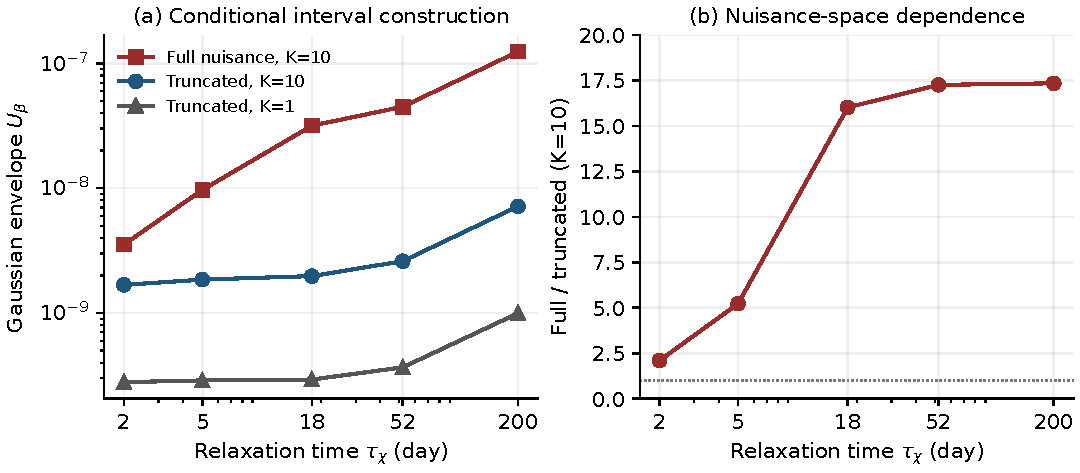
\includegraphics[width=\linewidth]{figures/conditional-intervals.pdf}
\caption{Imported from prior work. Stored interval envelopes and nuisance-space dependence. Left: K=1 and K=10 truncated constructions and the K=10 full-space scenario. Right: the full/truncated K=10 ratio. Connecting lines guide the eye; they do not certify unsampled lag or phase values. These are normalized-coefficient intervals, not universal SEP exclusions.}
\label{fig:intervals}
\end{figure}

\subsection{Coverage of the interval
construction}\label{coverage-of-the-interval-construction}

\textbf{Imported from prior work.} A registered experiment uses 8192
independent realizations per condition, 18 preselected lag/origin cells
and nine amplitudes (0, \(\pm2\), \(\pm5\), \(\pm20\) and \(\pm50\)
full-space unit-noise \(\sigma\)). The stresses are omitted means of
norm 3, 10 or 30 and extra Fourier modes 31--60, with spectral variance
proportional to \(j^{-4}\) normalized to weighted RMS 0.25 or 1. Table 2
reports pointwise coverage minima.

\begin{table}[htbp]
\centering
\caption{Imported from prior work. Minimum pointwise coverage of the K=1 U construction across tested cases. Each condition has 8192 realizations. Minima are descriptive, not simultaneous guarantees. Estimated covariance is a separately registered follow-through; dashes denote conditions not rerun for that estimator.}
\label{tab:coverage}
\begin{tabular}{l r r r r}
\toprule
Generating condition & Trunc. diag. & Full diag. & Oracle GLS & Est. GLS\\
\midrule
White noise & 0.9468 & 0.9481 & 0.9481 & 0.9473\\
Omitted mean, norm 3 & 0.0956 & 0.9481 & 0.9481 & --\\
Omitted mean, norm 10 & 0 & 0.9481 & 0.9481 & --\\
Omitted mean, norm 30 & 0 & 0.9481 & 0.9481 & --\\
Extra Fourier RMS 0.25 & 0.9310 & 0.7469 & 0.9485 & 0.9471\\
Extra Fourier RMS 1 & 0.8132 & 0.5825 & 0.9490 & 0.9459\\
\bottomrule
\end{tabular}
\end{table}

\textbf{Imported from prior work.} Truncation fails under omitted means,
and diagonal weighting fails under correlated extra Fourier power; the
oracle GLS control, which uses the generating covariance, restores
approximately nominal coverage. A follow-through registered after those
outcomes estimates \(C=\sigma^2(I+a^2LL^T)\) by restricted maximum
likelihood (REML) \cite{patterson1971reml}, a simple form of the
correlated-noise likelihoods used in pulsar timing
\cite{vanhaasteren2013noise}, where the columns of L are the extra
Fourier modes and a is their amplitude, the same fixed family that
generates the stress; across 486 conditions the minimum K=1 coverage is
7749/8192=0.945923. A truncated pointwise K=10 interval also has a
0/8192 stress case, while separately registered complete-grid tests at
lags 2 and 200 days give K=10 coverage of at least 511/512 in every
tested scenario. These are Monte Carlo results within the prescribed
covariance families, not an independently validated astrophysical noise
model.

\subsection{Information left after derivative and fast-spectrum
comparators}\label{information-left-after-derivative-and-fast-spectrum-comparators}

\textbf{Imported from prior work.} After full nuisance removal and
covariance whitening at the fixed amplitudes \(a=0,0.0831611,1\) (the
middle value from local REML fits to the stored residuals), the
six-carrier response maps have rank six and condition numbers
98.19--124.82. The retained information of a comparator is the Fisher
information for \(\beta\) after co-fitting the comparator's columns,
relative to co-fitting only the instantaneous column. Its minimum over
six lags and three specified phase sets (zero phases, one fixed
independent set, and the leading physical phases of Section 4, all with
unit carrier amplitudes) is 0.005389 at N=1, \(6.29\times10^{-5}\) at
N=2, \(1.17\times10^{-5}\) at N=3, and \(4.63\times10^{-6}\) at N=4; the
last widens the unit-noise standard error by about 465 times. The
even-only comparator \(\{0,2,4\}\) retains at least 0.0311. Mathematical
noninterpolation can therefore leave very little measurable information.
\textbf{Proven.} At N=5 the information is exactly zero by Theorem 1;
numerical residuals between \(5.4\times10^{-30}\) and
\(5.3\times10^{-25}\) are rounding error around that identity.
\textbf{Imported from prior work.} Projected through the same maps, the
inequality of Equation (\ref{eq:gap-witness}) gives a positive distance
witness for every tested lag with the explicitly illustrative
\(\Lambda=10\omega_{\rm in}\) (SM Section 5.6). This is a conditional
discrimination calculation, not a measured gap.

\subsection{Physical drive and simultaneous
inference}\label{physical-drive-and-simultaneous-inference}

\textbf{Imported from prior work.} With the runtime's parameter set, the
leading physical drive of Equation (\ref{eq:physical-drive}) has
\(U_*=1.74999156\times10^{-10}\), normalized amplitudes
\((0.24394925,0.69195682,0.06409393)\), and the phases implied by the
pericenters of Section 4. Exact coplanar Kepler-potential grids give an
omitted-input RMS of 3.37427 percent of the leading-drive RMS; this is
not an omitted timing-error bound. \textbf{Proven.} Fitting all six
carrier coefficients \(\theta\) before a lag or phase is selected lets a
confidence region E for them be inverted through the drive map
\(\theta=W(\phi,\tau)b\), \(b=(c_Y,\beta)\): the physical lag section at
lag \(\tau\) is the set of b with \(W(\phi,\tau)b\in E\), and this
controls continuous phase/lag selection within the declared mean model.
\textbf{Imported from prior work.} A six-coefficient REML region
calibrates a quadratic threshold of 12.8241766 from 8192 draws at each
\(a=0,0.25,1,4\), frozen before independent validation, whose inclusion
rates are 0.951660, 0.954346, 0.952759 and 0.954102; these support the
specified procedure, not every astrophysical noise process or
intermediate covariance. The recorded data's six-coefficient statistic,
16.3525, lies above that threshold (nominal chi-square p of about 0.012
for six degrees of freedom), so the data reject vanishing carrier
coefficients. This test differs from the unit-drive scan of Section 5.2
(p=0.26) in statistic, template and covariance: it tests all six carrier
coefficients at once. The best fit within the physical plane leaves a
statistic of 12.84 at 2 days and 14.39--14.59 at the other five
evaluated lags. Every evaluated physical lag section is therefore empty:
at these six lags, no instantaneous term plus single relaxation driven
by the leading physical drive reproduces the carrier coefficients at the
calibrated 95 percent level, and no interval on \(\beta\) or EOS-matched
bound follows. The 2-day rejection is marginal: the frozen threshold is
the largest of four calibration order statistics (12.27--12.82), each
with a Monte Carlo standard error near 0.13, although 12.84 exceeds all
four and the nominal chi-square value 12.59. \textbf{Proven.} The
rejection is robust for the equal-charge realization of Section 4, which
has \(\beta\ge0\). The statistic is a convex quadratic in b, the
\(\beta=0\) line lies in every section, and the unconstrained
\(\widehat\beta\) is negative at five lags and \(7.4\times10^{-12}\) at
18 days; so with \(\beta\ge0\) every section minimum is at least the
18-day value, 14.59. \textbf{Conjectural.} These results use the
archived timing derivatives, which Section 5.6 shows to be uncertain. At
the evaluated lags the excess is not explained by a response to this
drive, so it gives no evidence for relaxation; most of it lies in
directions that the drive does not span, and it is not attributed.
Timing-model mismatch at the orbital carriers, the derivative errors of
Section 5.6, the omitted drive terms and covariance misspecification are
candidates that this analysis does not separate.

\subsection{Limits of the stored
record}\label{limits-of-the-stored-record}

\textbf{Imported from prior work.} At \(\tau_\chi=500\) days,
one-per-mille settling of a transient requires 3453.88 days, longer than
the stored observing span. On the stored sampling, 0.7984--0.9973 of an
exponential input's norm lies outside the constant-plus-six-periodic
input span across the tested lags; this is input independence, not a
timing response. Dedicated live transient columns at \(\tau=2,52,500\)
days pass a registered 5-percent convergence gate. Co-fitting the
measured transient changes the physical-drive \(\beta\) standard errors
by factors 0.999998--1.00742 across the nine tested lag/covariance
combinations; this does not certify every lag, large initial amplitudes,
or coverage after adding that coefficient.

\textbf{Imported from prior work.} Recomputing the 28 timing derivatives
at half the archived steps leaves both nuisance matrices at rank 90 but
gives a maximum principal sine of 0.999913, changes the physical-drive
standard errors by factors 0.7858--0.8722 and shifts the estimates, so a
rigorous derivative-error budget remains unavailable. Among the 201
pulse-count assignments with at most two nonzero \(\pm1\) turn steps on
the ten longest gaps, the weakest is a single step at a 223.37-day gap,
with minimum chi-square changes 27.9406, 11.6183 and 0.152887 at
\(a=0,0.0831611,1\). Its unconstrained linear compensation implies
eccentricities above one and is rejected as a physical fit; this does
not exclude a different nonlinear solution. SM Sections 5.5--5.10 record
these audits in full.

\section{Discussion}\label{discussion}

\textbf{Proven.} Finite-order static representation and dynamical
identifiability are different questions. A settled single pole escapes a
restricted derivative comparator, but finitely many carriers are
interpolated once enough coefficients are admitted (Theorem 1), and
nuisance freedom can erase the remaining functional distinction.
Positivity with a rate gap restores a comparator restriction, and two
calibrated samples can identify one observable pole, but not the number
of internal variables behind it.

\textbf{Counterexample candidate.} The physical target is a shared
transfer relation with known drive and constrained projection, tested
against an explicitly bounded comparator. The one-state model is one
realization; hereditary kernels, multiple states, nonlinear thresholds
and other sectors remain separate possibilities.

\textbf{Imported from prior work.} For our stored J0337 analysis, the
interval on the relaxation coefficient depends strongly on the retained
nuisance span, and calibrated inference is available within specified
covariance families. At six evaluated lags between 2 and 500 days, the
recorded carrier coefficients carry an excess that the leading physical
drive, with or without a single relaxation, does not reproduce; no
relaxation is detected. The physical-drive fits have standard errors of
\(3.5\times10^{-10}\) to \(1.7\times10^{-9}\) in \(\beta\), about 2 to
10 in \(B=\beta/U_*\). The measured derivative sensitivity and the
unphysical full pulse compensation keep the analysis from serving as an
empirical constraint.

\textbf{Conjectural.} SM Section 4.6 works through one internal state of
the inner white dwarf of the triple, the scalar-driven displacement of
its own matter, in a specified weak-field scalar-tensor model. A scalar
pulse leaves in the displaced matter a transient retarded monopole
signal. Under the stated assumptions, which include linear response,
\(|a_p|\le1\) and an outer-companion charge near the Cassini limit, its
structural modulation of the pair factors at orbital timescales lies
about eight orders of magnitude below the smallest stored Section 5
scale. A prescribed layer-by-layer relaxation estimate, not a
non-adiabatic calculation, gives contributions from the scanned layers
of \(4.0\times10^{-9}\) and \(3.3\times10^{-7}\) of the structural term
at the inner and outer orbital frequencies. The scan stops at a thermal
time of \(10^{13}\) s; deeper layers have an uncomputed relaxation
strength, so these partial sums do not bound the total lag without the
tail condition stated in SM Section 4.6. These responses enter the
pulsar-inner and inner-outer pair factors, not the common modulation of
Section 4. The white dwarfs' instantaneous zero-lag responses could
reach the smallest stored scale only for \(|a_p|\gtrsim0.5\), which the
static SEP limits allow only if \(|a_o|\lesssim5\times10^{-6}\); they
are not lags. Neither timing response was computed, so this is a scale
comparison, not an exclusion. Other internal states of the white dwarfs,
and the neutron-star charge of Section 4, remain open.

\textbf{Conjectural.} A physically calibrated exclusion still requires
numerical EOS-to-body matching, control of omitted drive/force terms, a
reliable derivative space and an adequate astrophysical likelihood. The
fast-rate gap remains an unestablished physical premise, and no
mechanism that produces a relaxation at the stored 2--500-day lags with
a coupling B of that size is identified here. The result is a set of
identifiability boundaries and a conditional application, not a
universal empirical SEP bound.

\section*{Use of AI tools}\label{use-of-ai-tools}
\addcontentsline{toc}{section}{Use of AI tools}

This work used AI agents substantively, under the author's direction and
responsibility. Coding agents built on Claude Opus 5.5 (Anthropic, run
through Claude Code) and GPT-6-Astra (OpenAI, run through the Codex
command-line tool) wrote and ran most of the analysis, stellar-structure
and verification code, carried out the computations reported here, and
drafted and revised manuscript text, including scientific claims and
explanations. GPT-6-Astra, Claude Opus 5.5 and Claude Fable 5.1
(Anthropic, run as a Claude Code subagent) independently reviewed drafts
of the white-dwarf calculation (SM Section 4.6) in several rounds and
the complete manuscript before submission; their reports and the
responses are archived in the repository. The author set the research
questions, the acceptance criteria and the claim labels, and checked the
AI output against the stored numerical records, the SHA-256-bound
manifests, symbolic checks, the verification program named below and
these reviews.

\section*{Statements and
declarations}\label{statements-and-declarations}
\addcontentsline{toc}{section}{Statements and declarations}

\subsection*{Competing interests}\label{competing-interests}
\addcontentsline{toc}{subsection}{Competing interests}

The author declares no competing interests.

\subsection*{Funding}\label{funding}
\addcontentsline{toc}{subsection}{Funding}

The author received no external funding for this research.

\subsection*{Author contributions}\label{author-contributions}
\addcontentsline{toc}{subsection}{Author contributions}

J.K. conceived and directed the study, set the research questions and
acceptance criteria, checked the results against archived numerical
records and verification tests, and reviewed and approved the
manuscript. AI assistance with coding, computation, drafting and
internal review is disclosed in the Use of AI tools section. J.K. takes
responsibility for the work.

\section*{Data and code availability}\label{data-and-code-availability}
\addcontentsline{toc}{section}{Data and code availability}

The public timing release is cited as a dataset
\cite{voisin2025release}. The manuscript and SM sources, code, notes,
manifests and numerical results are available in the public snapshot
tagged \path{grg-submission-2026-09-28} at
\url{https://github.com/lpaiu-cs/self-mass-unobservability}. The
accompanying \path{paper/revision-manifest.json} identifies this
revision's inputs by SHA-256, and
\path{output/submission/grg/manifest.json} binds the submission files.
Binary runtime arrays, about 50 GB in total, exceed the hosting limits
and are not deposited; the manifests identify them by SHA-256, and they
are available from the author on request. Commit identifiers cited in
the SM refer to the author's full repository history, of which the
public repository holds a snapshot; \path{PUBLIC_SNAPSHOT.md} there
states what the snapshot omits.

Online Resource 1 (ESM\_1.pdf): complete technical account, static
operator catalog, derivations, numerical audits and white-dwarf
calculation. The SM source is
\path{output/submission/grg/supplement.md}. It contains the static
operator catalog, all derivations, the full audits with their
registration commits and reproduction commands, and the white-dwarf
calculation with a map from each result to its manifest. The public JSON
record \path{outputs/research-completion/public-inference.json} supplies
the six fitted coefficients, their precision matrix, the physical-drive
map and the frozen threshold. With NumPy,
\path{verification/replay_public_inference.py} reproduces the omnibus
statistic and the six physical lag sections from this record without
private arrays. It does not validate the timing derivatives or
recalibrate coverage. The broader
\path{verification/verify_unified_paper.py} also checks finite-carrier
interpolation, stored audits, Tables 1 and 2, and input hashes; it
requires the omitted arrays but does not invoke Nutimo. Outputs
superseded by the periastron-convention correction of Sections 4 and 5
are kept in
\path{outputs/research-completion/withdrawn-periastron-convention/}.

\bibliographystyle{unsrtnat}
\bibliography{references}

\end{document}
